\subsection{Use case} \label{sec:usecase} 
På baggrund af systembeskrivelsen samt opstillede krav er der udarbejdet et use case diagram, der beskriver app'ens funktioner. Af use case diagrammet på \autoref{fig:usecase} ses systemet, app til KOL-patienter, samt de forskellige use cases og aktører, der interagerer med systemet. KOL-patienten er den primære aktør, som kan tilgå alle use cases.  Database og andre KOL-patienter er sekundære aktører og kan kun tilgå enkelte use cases. Sundhedspersonalet har kun adgang til data via en database. 

\begin{figure} [H]
\centering
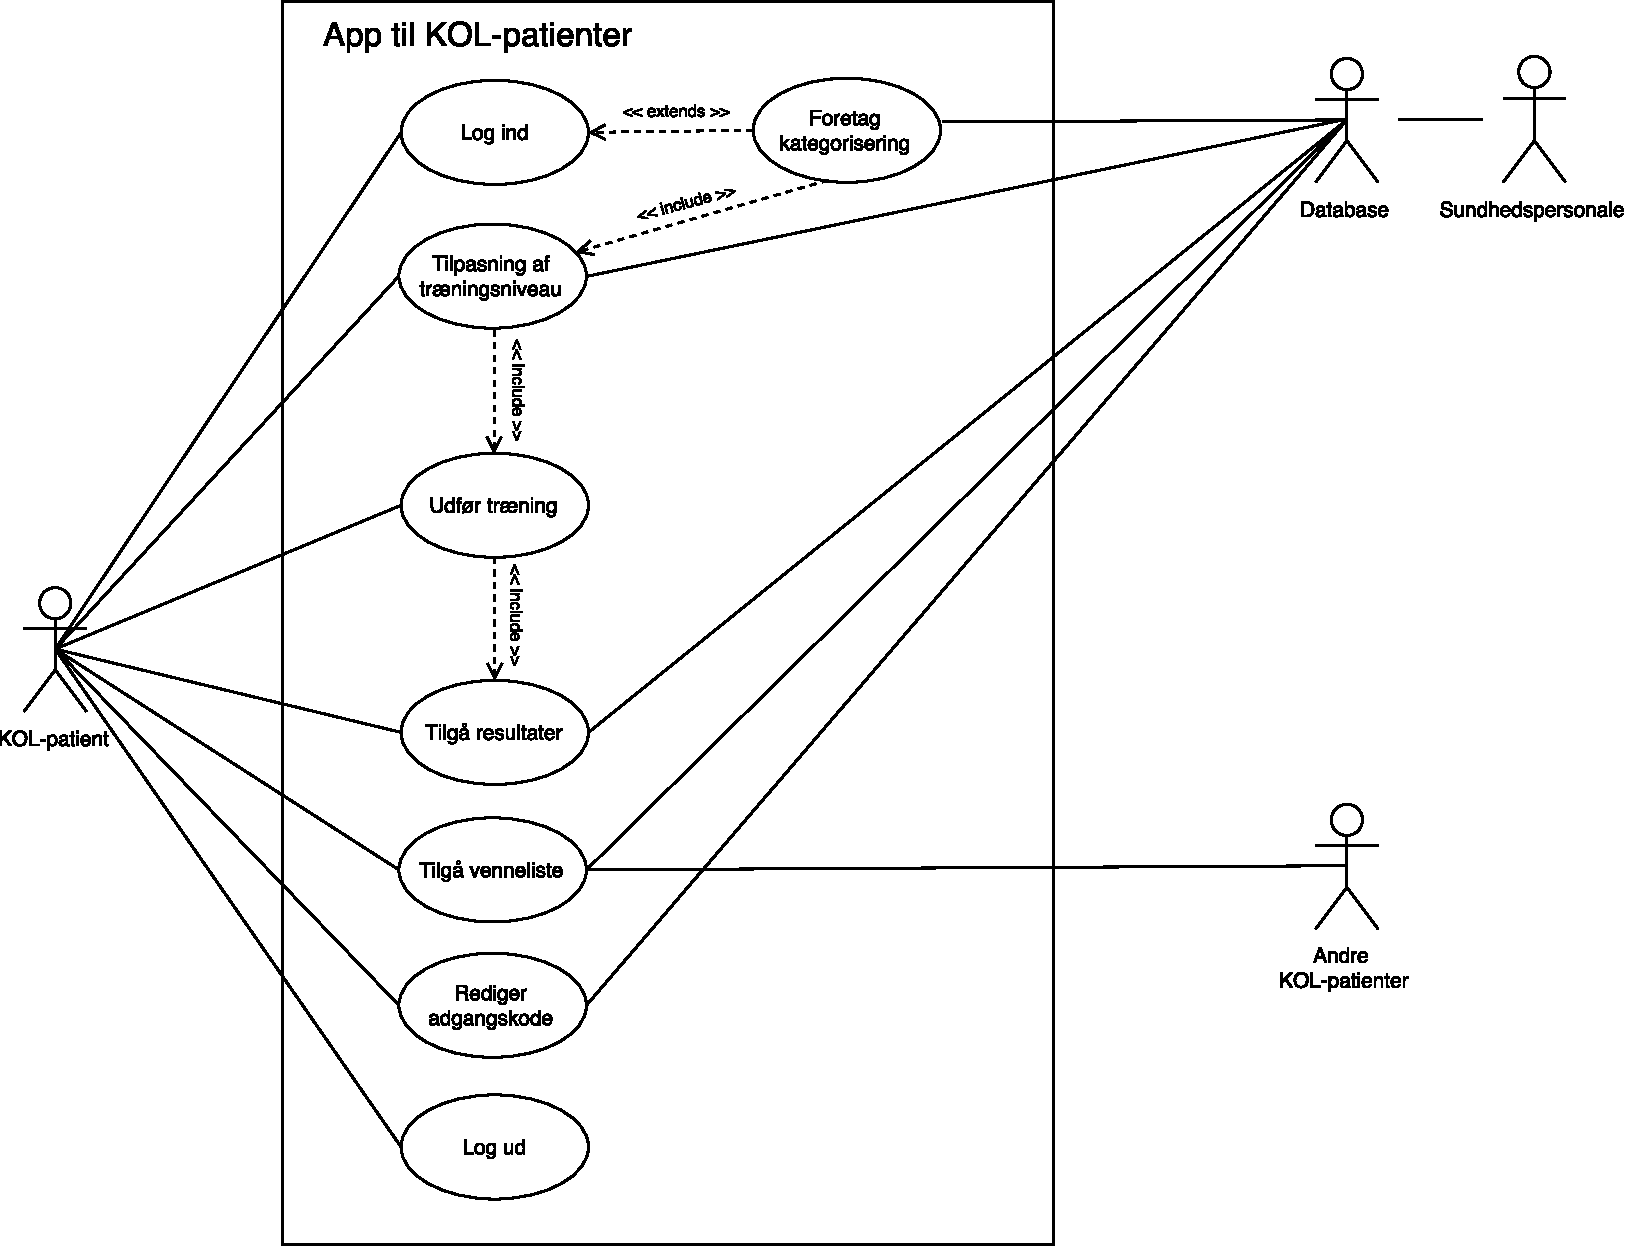
\includegraphics[width=0.9\textwidth]{figures/aktivitetsdiagram/Usecase}
\caption{Use case diagram for app til KOL-patienter}
\label{fig:usecase}
\end{figure}

\noindent
KOL-patienter skal \textit{Log ind} i app'en via medlemsID og adgangskode. Første gang de logger ind skal de \textit{Foretag kategorisering}. Denne kategorisering gemmes efterfølgende i en database.
Hvis kategoriseringen er foretaget har brugere adgang til en hovedmenu, hvorfra de kan vælge at udføre træning, tilgå resultater, tilgå venneliste, redigere adgangskode og logge ud. 

Vælger brugeren, at \textit{Udføre træning} tilpasses træningsniveauet før selve træningen kan påbegyndes ud fra \textit{Tilpasning af træningsniveau}, der vurderes på baggrund af kategoriseringen, daglig helbredstilstand samt evaluering af tidligere træninger. 

Efter træningen skal brugere evaluere træningen, og de kan efterfølgende tilgå deres  resultater. Evaluering og resultater fra træningen gemmes efterfølgende i en database. Brugere kan \textit{Tilgå resultater}, der vises som virtuelle belønninger, som opnås på baggrund af udførte træninger. 

Brugere kan via \textit{Tilgå venneliste} tilgå andre KOL-patienters virtuelle belønninger, hvilket medvirker til, at brugere kan motivere hinanden til at udføre træning. 

Brugere kan \textit{Redigere adgangskode}, da det skal være muligt for brugeren at ændre adgangskoden til en personlig adgangskode. Hvis der foretages ændringer gemmes disse efterfølgende i databasen.
Brugeren kan \textit{Log ud} af app'en, hvis dette ønskes. 

%På baggrund af systembeskrivelsen samt opstillede krav er der udarbejdet et use case diagram, der beskriver app'ens funktioner. Af use case diagrammet på \autoref{fig:usecase} ses systemet, app til KOL-patienter, samt de forskellige use cases og aktører, der interagerer med systemet. KOL-patienten er den primære aktør, som kan tilgå alle use cases. Målinger, database, sundhedspersonale og andre KOL-patienter er sekundære aktører og kan kun tilgå enkelte use cases. 
%
%\begin{figure} [H]
%\centering
%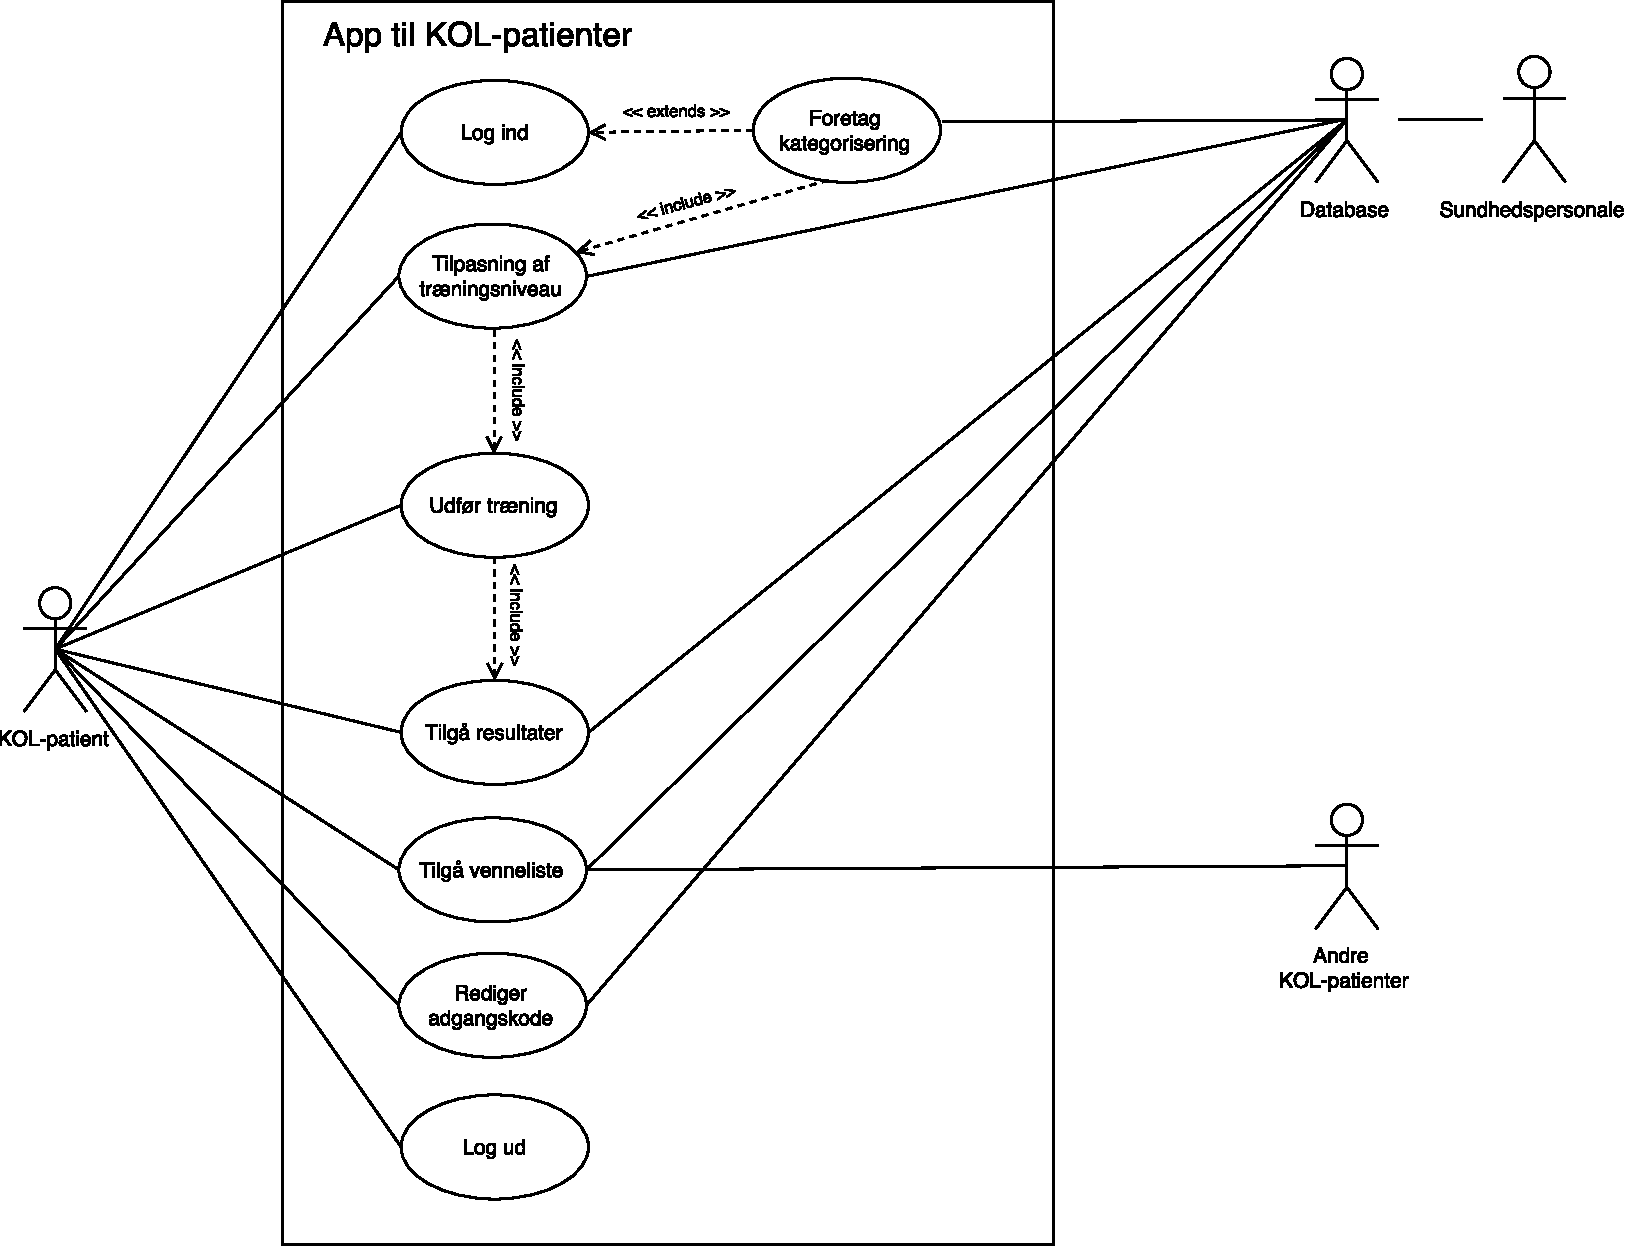
\includegraphics[width=0.9\textwidth]{figures/aktivitetsdiagram/Usecase}
%\caption{Use case for app til KOL-patienter}
%\label{fig:usecase}
%\end{figure}
%
%\noindent
%Efter KOL-patienter er logget ind i app'en har de adgang til en hovedmenu, hvorfra brugere kan vælge at redigere brugeroplysninger, udføre træning, se resultater og venneliste. 
%
%I \textit{Redigering af brugeroplysninger} kan brugere redigere deres adgangskode og kategorisering. Det skal være muligt for brugeren at ændre adgangskoden til en personlig adgangskode, da de ved registrering får en randomiseret adgangskode udleveret. Derudover skal det være muligt at ændre kategoriseringen af KOL, da deres tilstand grundet KOL kan ændres. Hvis der foretages ændringer gemmes disse efterfølgende i databasen. 
%
%\textit{Valg af træningsniveau} tilpasses individuelt ud fra \textit{Patientstatus}, der vurderes ud fra \textit{Kategorisering}, \textit{Daglig helbredstilstand} samt \textit{Evaluering af træning}.
%Under \textit{Træning} kan eksterne måleenheder tilkobles systemet, således målinger kan opsamles. Ved en udført træning startes en nedtælling, som efter 24 timer viser en \textit{Notifikation} med henblik på at motivere brugeren til træning. Hvis brugeren benytter app'en førend de 24 timer er gået, nulstilles nedtællingen.
%Efter udført træning samt evaluering gemmes patientens status, træningsresultater samt målinger i \textit{Resultater} og databasen. 
%Brugere kan tilgå samtlige resultater, som visualiseres ved grafisk udvikling, en kalender samt belønninger. Sundhedspersonalet kan kun tilgå udviklingen af brugerens træning. Brugerne skal via \textit{Venneliste} kunne tilgå andres belønninger, hvilket medvirker til, at brugere kan motiveres til at udføre træning. Efter hver handling returneres brugeren til hovedmenuen.